% ch05 Hartree–Fock approximation (书页 31–36 / 分册p001–p006)
% 第5章 Hartree–Fock approximation
\chapter{哈特里–福克近似}

在上一章中我们证明了，固体中相互作用电子系的哈密顿量可以写成二次量子化形式
\begin{equation*}
\widehat{H}_{\rm e}=\sum_{\nu\lambda}\langle\nu|\widehat{h}(1)|\lambda\rangle a_\nu^\dagger a_\lambda+\frac{1}{2}\sum_{\nu\lambda\alpha\beta}\langle\nu\lambda|\frac{e^2}{|\mathbf{r}_1-\mathbf{r}_2|}|\alpha\beta\rangle a_\nu^\dagger a_\lambda^\dagger a_\beta a_\alpha,
\tag{5.1}
\end{equation*}
其中 $\widehat{h}(1)=\widehat{\mathbf{p}}_1^2/2m+\widehat{V}_{\rm ion}(\mathbf{r}_1)$，希腊字母标记单粒子轨道。本章我们对关联电子问题引入哈特里–福克（Hartree--Fock）近似。这一近似的基本假设是：基态与无相互作用体系的基态相同，能量则取为该态中的期望值。

\section{无相互作用极限}

我们先用二次量子化重新表述无相互作用问题。在 $T=0$ 的无相互作用电子问题中，直到费米能级为止的所有动量态都是双重占据的。因此，我们把填满的费米海的基态波函数表示为
\begin{equation*}
|\psi_0\rangle=|\mathbf{p}_0\uparrow,\mathbf{p}_0\downarrow,\ldots,\mathbf{p}_{\rm F}\uparrow,\mathbf{p}_{\rm F}\downarrow\rangle=a_{\mathbf{p}_0\uparrow}^\dagger a_{\mathbf{p}_0\downarrow}^\dagger\ldots a_{\mathbf{p}_{\rm F}\uparrow}^\dagger a_{\mathbf{p}_{\rm F}\downarrow}^\dagger|0\rangle.
\tag{5.2}
\end{equation*}
我们用动量态 $\mathbf{p}$ 的粒子数算符 $\widehat{n}_{\mathbf{p}\sigma}$ 作用在基态波函数上，求出第 $p$ 能级的占据数：
\begin{equation*}
\widehat{n}_{\mathbf{p}\sigma}|\psi_0\rangle=n_{\mathbf{p}\sigma}|\psi_0\rangle.
\tag{5.3}
\end{equation*}
借助这一等式，我们把动能的期望值
\begin{align*}
\langle\widehat{T}\rangle&=\langle\psi_0|\sum_{\mathbf{p},\sigma}\frac{p^2}{2m}\widehat{n}_{\mathbf{p}\sigma}|\psi_0\rangle\\
&=2\sum_{p=0}^{p_{\rm F}}\frac{p^2}{2m}
\tag{5.4}
\end{align*}
化简，得到标准的自由粒子结果
\begin{equation*}
\langle\widehat{T}\rangle=\frac{3}{5}\frac{p_{\rm F}^2}{2m}N.
\tag{5.5}
\end{equation*}

在计算离子项的期望值时，我们必须求出形如 $\langle\psi_0|a_{\mathbf{p}\sigma}^\dagger a_{\mathbf{p}'\sigma}|\psi_0\rangle$ 的表达式。由于 $p<p_{\rm F}$ 的所有态都已填满，对 $p<p_{\rm F}$ 有 $a_{\mathbf{p}\sigma}^\dagger|\psi_0\rangle=0$；类似地，若 $p'>p_{\rm F}$ 则 $a_{\mathbf{p}'\sigma}|\psi_0\rangle=0$。当 $a_{\mathbf{p}\sigma}^\dagger a_{\mathbf{p}'\sigma}$ 作用在 $|\psi_0\rangle$ 上时，产生的新态与 $\psi_0$ 至多相差两个单粒子态。由于动量本征态的正交性，该新态与 $|\psi_0\rangle$ 的交叠必为零——当然，除非 $\mathbf{p}=\mathbf{p}'$、$\sigma=\sigma'$：
\begin{equation*}
\langle\psi_0|a_{\mathbf{p}\sigma}^\dagger a_{\mathbf{p}'\sigma}|\psi_0\rangle=\delta_{\mathbf{p}\mathbf{p}'}n_{\mathbf{p}\sigma}.
\tag{5.6}
\end{equation*}
因此，
\begin{equation*}
\langle\widehat{V}_{\rm ion}\rangle=\sum_{\mathbf{p},\sigma}n_{\mathbf{p}\sigma}V_{\rm ion}(0),
\tag{5.7}
\end{equation*}
其中
\begin{equation*}
V_{\rm ion}(0)=\frac{1}{V}\int{\rm d}\mathbf{r}\,V_{\rm ion}(\mathbf{r}).
\tag{5.8}
\end{equation*}
最终结果是
\begin{equation*}
\langle\widehat{H}_1\rangle=2\sum_{p<p_{\rm F}}\left(\frac{p^2}{2m}+V_{\rm ion}(0)\right).
\tag{5.9}
\end{equation*}

作为通往哈特里–福克近似的第一步，把这个结果改写到位置空间是有益的。为了在位置空间中重新表述我们的问题，我们反演傅里叶变换，把动量产生算符写成
\begin{equation*}
a_{\mathbf{p}\sigma}^\dagger=\int{\rm d}\mathbf{r}\,\frac{{\rm e}^{{\rm i}\mathbf{p}\cdot\mathbf{r}/\hbar}}{\sqrt{V}}\psi_\sigma^\dagger(\mathbf{r}).
\tag{5.10}
\end{equation*}
在哈密顿量中代入式 (5.10) 的二次量子化算符并对 $p$ 求和，我们得到
\begin{align*}
\widehat{H}_1&=\sum_\sigma\int{\rm d}\mathbf{r}\left[-\frac{\hbar^2}{2m}\psi_\sigma^\dagger(\mathbf{r})\nabla^2\psi_\sigma(\mathbf{r})+\psi_\sigma(\mathbf{r})V_{\rm ion}(\mathbf{r})\psi_\sigma(\mathbf{r})\right]\\
&=\sum_\sigma\int{\rm d}\mathbf{r}\left[\frac{\hbar^2}{2m}|\nabla\psi_\sigma|^2+\widehat{n}_\sigma(\mathbf{r})V_{\rm ion}(\mathbf{r})\right]:
\tag{5.11}
\end{align*}
多体系统的动能算符正比于算符 $|\nabla\psi_\sigma|^2$；类似地，单体势项以密度算符 $\psi_\sigma^\dagger(\mathbf{r})\psi_\sigma(\mathbf{r})$ 加权。\footnote{译注：原文式 (5.11) 第一行 $V_{\rm ion}$ 前的场算符印作 $\psi_\sigma(\mathbf{r})$；按本意（对照本式第二行的密度算符 $\widehat{n}_\sigma(\mathbf{r})=\psi_\sigma^\dagger\psi_\sigma$ 及下文）应为产生算符 $\psi_\sigma^\dagger(\mathbf{r})$，此处照原文排印。}

把二次量子化表达式 (5.11) 与式 (5.1) 所定义的轨道基下 $\widehat{H}_1$ 的期望值联系起来颇有启发：
\begin{align*}
\langle\widehat{H}_1\rangle&=\sum_\nu\langle\nu|\widehat{h}(1)|\nu\rangle n_\nu\\
&=\sum_{\nu\,{\rm (occ.)}}\int\left[\frac{\hbar^2}{2m}|\nabla\phi_\nu|^2+\phi_\nu^*(\mathbf{r})V_{\rm ion}(\mathbf{r})\phi_\nu(\mathbf{r})\right]{\rm d}\mathbf{r}.
\tag{5.12}
\end{align*}
梯度项与轨道密度项同式 (5.11) 中的对应项一一相应。唯一的差别是：二次量子化表达式 (5.11) 中用产生或湮灭粒子的场算符 $\psi_\sigma(\mathbf{r})$ 取代了单粒子轨道。

\section{哈特里–福克近似}

现在转向 $H$ 的二体部分。我们还须计算的附加项是
\begin{align*}
\langle\widehat{H}_2\rangle&=\langle\psi_0|\widehat{V}_{\rm ee}|\psi_0\rangle\tag{5.13}\\
&=\frac{1}{2}\sum_{\alpha,\beta,\nu,\lambda}\langle\nu|\langle\lambda|\frac{e^2}{|\mathbf{r}_1-\mathbf{r}_2|}|\alpha\rangle|\beta\rangle\langle a_\nu^\dagger a_\lambda^\dagger a_\beta a_\alpha\rangle,
\tag{5.14}
\end{align*}
其中 $\langle\ldots\rangle=\langle\psi_0|\ldots|\psi_0\rangle$，而 $\langle r|\psi_0\rangle$ 是轨道基下的基态波函数。我们把自旋指标隐含在 $\alpha,\beta,\ldots$ 之中；不过请记住，指标 $\nu$ 所带的自旋与 $\alpha$ 的相同，而指标 $\lambda$ 所带的自旋与 $\beta$ 的相同。

为化简式 (5.13)，我们必须学会如何在轨道基态 $|\psi_0\rangle$ 中计算二次量子化算符串的期望值。先考虑态 $|n_\alpha n_\beta\rangle$ 中的期望值。利用关系 $a_\alpha|n_\alpha\rangle=\sqrt{n_\alpha}\,|n_\alpha-1\rangle$，我们有
\begin{equation*}
\langle n_\alpha n_\beta|a_\nu^\dagger a_\lambda^\dagger a_\beta a_\alpha|n_\alpha n_\beta\rangle=\sqrt{n_\alpha n_\beta}\,\langle n_\alpha n_\beta|a_\nu^\dagger a_\lambda^\dagger|n_\alpha-1,n_\beta-1\rangle.
\tag{5.15}
\end{equation*}
该量仅在 $\nu=\beta$、$\lambda=\alpha$，或 $\nu=\alpha$、$\lambda=\beta$ 时才不为零。由于算符 $a_\alpha$ 的反对易关系，这两种情形给出的贡献相差一个负号。于是我们得到
\begin{equation*}
\langle n_\alpha n_\beta|a_\nu^\dagger a_\lambda^\dagger a_\beta a_\alpha|n_\alpha n_\beta\rangle=(\delta_{\nu\alpha}\delta_{\lambda\beta}-\delta_{\nu\beta}\delta_{\lambda\alpha})n_\alpha n_\beta,
\tag{5.16}
\end{equation*}
而对式 (5.2) 给出的基态，则有
\begin{equation*}
\langle a_\nu^\dagger a_\lambda^\dagger a_\beta a_\alpha\rangle=(\delta_{\nu\alpha}\delta_{\lambda\beta}-\delta_{\nu\beta}\delta_{\lambda\alpha})\langle\widehat{n}_\alpha\rangle\langle\widehat{n}_\beta\rangle.
\tag{5.17}
\end{equation*}
分解这类期望值的一般规则由威克（Wick）给出 [W1950]：他证明了 $\langle a_\nu^\dagger a_\lambda^\dagger\ldots a_l^\dagger a_\rho a_\alpha\ldots a_\gamma\rangle$ 等于所有收缩之和，每项的符号由把被收缩的算符两两排到相邻位置所需的粒子交换次数决定。注意：两个算符被收缩时，它们的指标便变得相同。

有了这个结果，我们把 $\langle\widehat{H}_2\rangle$ 改写成两个积分之和：
\begin{align*}
\langle\widehat{H}_2\rangle&=\frac{1}{2}\sum_{\lambda,\nu}\langle\nu|\langle\lambda|\frac{e^2}{|\mathbf{r}_1-\mathbf{r}_2|}|\nu\rangle|\lambda\rangle n_\lambda n_\nu-\frac{1}{2}\sum_{\lambda,\nu}\langle\nu|\langle\lambda|\frac{e^2}{|\mathbf{r}_1-\mathbf{r}_2|}|\lambda\rangle|\nu\rangle n_\lambda n_\nu\\
&=\frac{1}{2}\sum_{\lambda,\nu\,{\rm (occ.)}}\left(U_{\nu\lambda}-\delta_{\sigma_\nu\sigma_\lambda}J_{\nu\lambda}\right).
\tag{5.18}
\end{align*}
直接库仑相互作用
\begin{equation*}
U_{\nu\lambda}=\int{\rm d}\mathbf{r}_1\,{\rm d}\mathbf{r}_2\,|\phi_\nu(\mathbf{r}_1)|^2\frac{e^2}{|\mathbf{r}_1-\mathbf{r}_2|}|\phi_\lambda(\mathbf{r}_2)|^2,
\tag{5.19}
\end{equation*}
度量位于 $\mathbf{r}_1$ 与 $\mathbf{r}_2$ 处的两个电子之间的排斥；而交换相互作用
\begin{equation*}
J_{\nu\lambda}=\int{\rm d}\mathbf{r}_1\,{\rm d}\mathbf{r}_2\,\phi_\nu^*(\mathbf{r}_1)\phi_\lambda^*(\mathbf{r}_2)\frac{e^2}{|\mathbf{r}_1-\mathbf{r}_2|}\phi_\nu(\mathbf{r}_2)\phi_\lambda(\mathbf{r}_1),
\tag{5.20}
\end{equation*}
仅当自旋相同的电子交换空间坐标时才会出现。伴随交换项出现的负号导致自旋相同的电子之间存在有效吸引。这种吸引是海森堡（Heisenberg）铁磁性解释的基础。由电子服从的费米–狄拉克统计导出的泡利不相容原理（Pauli exclusion principle），使得在给定自旋的电子周围，同自旋电子的分布出现耗尽。这一耗尽通常称为“交换空穴”（exchange hole）[P1953]。

式 (5.12) 与式 (5.18) 合起来构成了 $\widehat{H}_{\rm e}$ 在态 $|\psi_0\rangle$ 中期望值的精确表达式。总哈特里–福克能量为
\begin{equation*}
E_{\rm HF}=\langle\widehat{H}_1\rangle+\frac{1}{2}\sum_{\lambda,\nu\,{\rm (occ.)}}[U_{\nu\lambda}-J_{\nu\lambda}].
\tag{5.21}
\end{equation*}
尚缺的细节是求出轨道 $\phi_\nu$ 与 $\phi_\lambda$ 的方法。为确定它们，我们在保持各 $\phi$ 归一化的约束条件下，对各 $\phi$ 变分以极小化基态能量 $E_{\rm HF}$。这一约束条件可以通过在极小化中引入拉格朗日乘子 $\epsilon_\nu$ 来施加：
\begin{equation*}
\frac{\delta E_{\rm HF}}{\delta\phi_\nu^*(\mathbf{r})}=\epsilon_\nu\frac{\delta}{\delta\phi_\nu^*(\mathbf{r})}\int{\rm d}\mathbf{r}'\,|\phi_\nu(\mathbf{r}')|^2.
\tag{5.22}
\end{equation*}
我们稍后讨论能量 $\epsilon_\nu$ 的物理意义。对式 (5.22) 完成变分，便得到著名的单粒子轨道 $\phi_\nu(\mathbf{r})$ 的哈特里–福克方程
\begin{equation*}
\begin{aligned}
&\left[\frac{-\hbar^2}{2m}\nabla^2+\widehat{V}_{\rm ion}(\mathbf{r})+\sum_\lambda\int{\rm d}\mathbf{r}'\,n_\lambda(\mathbf{r}')\frac{e^2}{|\mathbf{r}-\mathbf{r}'|}\right]\phi_\nu(\mathbf{r})\\
&\qquad-\sum_\lambda\int{\rm d}\mathbf{r}'\,\phi_\lambda^*(\mathbf{r}')\phi_\nu(\mathbf{r}')\frac{e^2}{|\mathbf{r}-\mathbf{r}'|}\phi_\lambda(\mathbf{r})=\epsilon_\nu\phi_\nu(\mathbf{r})
\end{aligned}
\tag{5.23}
\end{equation*}
在没有平移不变性时，这些变分方程可以迭代求解，直到求出一组自洽的轨道及相应的能量 $\epsilon_\nu$。

把式 (5.23) 乘以 $\phi_\nu^*(\mathbf{r})$ 并对 $\mathbf{r}$ 积分，我们得到单粒子能量 $\epsilon_\nu$ 的结果
\begin{equation*}
\epsilon_\nu=\langle\nu|h_1|\nu\rangle+\sum_{\lambda\,{\rm (occ.)}}(U_{\nu\lambda}-J_{\nu\lambda}).
\tag{5.24}
\end{equation*}

\begin{figure}[H]\centering
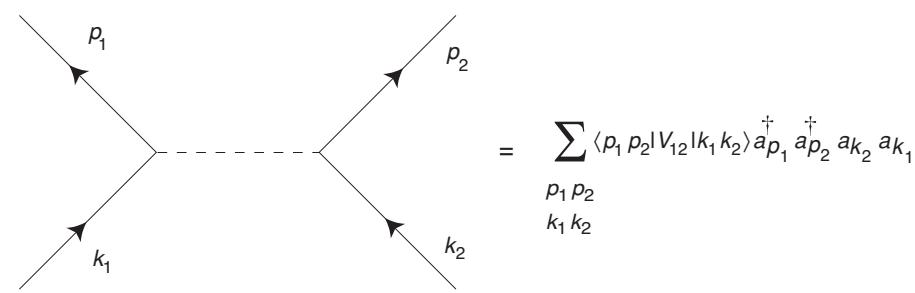
\includegraphics[width=0.8\textwidth]{figs/ch05/fig_5.1.jpg}
\caption*{图 5.1\quad 一般的二体相互作用}\label{fig:auto:5.1}
\end{figure}

由于这些能量包含与所有其他被占轨道中电子的相互作用，$\epsilon_\nu$ 不能简单地解释为轨道 $\nu$ 中电子的能量。事实上，如式 (5.21) 所表明的，总能量并不是这些单粒子能量的简单求和，而是
\begin{equation*}
E_{\rm HF}=\sum_{\nu\,{\rm (occ.)}}\epsilon_\nu-\frac{1}{2}\sum_{\lambda,\nu\,{\rm (occ.)}}(U_{\nu\lambda}-J_{\nu\lambda}).
\tag{5.25}
\end{equation*}
库普曼斯（Koopmans）[K1934] 指出，哈特里–福克单粒子能量 $\epsilon_\nu$ 正是把一个粒子添加到原先未被占据的轨道 $\nu$ 中所需的能量。考虑把一个额外电子加到一组已填满轨道之外原先空着的轨道 $\nu$ 上。由添加该粒子引起的哈特里–福克能量的改变为
\begin{equation*}
\delta E_{\rm HF}=E_{\rm HF}^{\rm new}-E_{\rm HF}=\langle\nu|h(1)|\nu\rangle+\sum_{\alpha\neq\nu}(U_{\nu\alpha}-J_{\nu\alpha})=\epsilon_\nu.
\tag{5.26}
\end{equation*}
同样，若移走一个电子，所得的哈特里–福克能量将简单地减少该电子原来所在轨道的能量。相当普遍地，从 $N$ 粒子系统变到 $N-1$ 粒子系统时，$\delta E_{\rm HF}=\epsilon_N=E_N^{\rm HF}-E_{N-1}^{\rm HF}$。库普曼斯定理断言：$-\epsilon_N$ 可以取作体系第一电离势的一个变分近似。对原子而言，库普曼斯定理预言的电离势与实验符合得相当好 [W1964]。

\section{图示}

在本书中，我们将始终把图形用作表示粒子间相互作用过程的启发性工具。图 5.1 画出了式 (5.13) 中的二体相互作用。前向箭头表示给定动量的粒子的传播，虚线表示两电子库仑相互作用。图 5.2 用图形表示出相互作用能、即式 (5.18) 中的各项。这里反向的线表示空穴的传播。

\begin{figure}[H]\centering
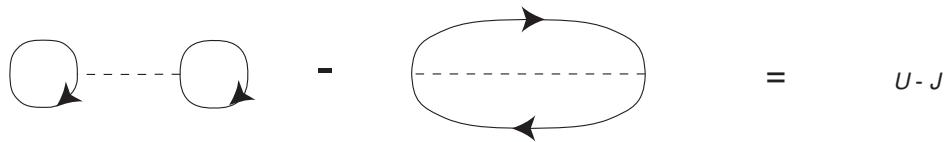
\includegraphics[width=0.85\textwidth]{figs/ch05/fig_5.2.jpg}
\caption*{图 5.2\quad 直接相互作用与交换相互作用}\label{fig:auto:5.2}
\end{figure}

\section*{习题}
\addcontentsline{toc}{section}{习题}

\textbf{习题 5.1}\quad 证明哈特里–福克能量可以写成
\begin{equation*}
E_{\rm HF}=\sum_{n=1}^{N}\epsilon_n,
\tag{5.27}
\end{equation*}
其中 $N$ 为单粒子轨道的数目，且
\begin{equation*}
\epsilon_n=\langle n|\widehat{H}_1|n\rangle+\sum_{\lambda=1}^{n}[U_{n\lambda}-J_{n\lambda}].
\tag{5.28}
\end{equation*}
试结合“真正的哈特里–福克能量不能写成单粒子能量之和”这一事实解释此结果。

\section*{参考文献}
\addcontentsline{toc}{section}{参考文献}

\begin{itemize}[leftmargin=2em,itemsep=0pt,parsep=0pt,label={}]
\item [K1934] T. Koopmans, \textit{Physica} \textbf{1}, 104 (1934). Interestingly, this theorem is Koopmans' only physics contribution. Immediately after publishing this work, he switched to economics, a field in which he later won the Nobel Prize.
\item [P1953] D. Pines, \textit{Phys. Rev.} \textbf{92}, 626 (1953).
\item [W1964] See A. C. Wahl, \textit{J. Chem. Phys.} \textbf{41}, 2600 (1964) for a failure of Koopmans' theorem in the molecule F$_2$.
\item [W1950] G.-C. Wick, \textit{Phys. Rev.} \textbf{80}, 268 (1950).
\end{itemize}
